

We now move to settings that are specific to supersingular curves.
We focus on the relations $\R[isog]$ and $\R[deg]$.
%, and later we briefly discuss the challenges of $\R[SIDH]$.
As mentioned in Section~\ref{sec:isog-graph} it suffices to consider elliptic curves defined over a finite field $\F_{p^2}$.
%, as we saw that any supersingular curve is isomorphic to one defined over a quadratic finite field.
Lacking a well behaved group action on the set of supersingular curves, we have to get more creative in order to define secure protocols.

Along with the SIDH key exchange, De Feo, Jao and Pl\^{u}t~\cite{DFJP14} sketched the first sigma protocol to prove knowledge of an isogeny between two supersingular curves over $\F_{p^2}$, provided $p$ is an ``SIDH prime''.
We start by presenting this simple protocol, which we refer to as DFJP.
We highlight some issues with its soundness and zero-knowledge, and explain how to fix them, following De Feo, Dobson, Galbraith and Zobernig~\cite{DFDGZ21}.
Then, we present a recent generalization of DFJP which applies to any characteristic and achieves statistical zero-knowledge~\cite{cryptoeprint:2022/1469}.
Finally, we discuss some open questions.


\subsection{The DFJP protocol}\label{sec:DFJP}

We are in the SIDH setting, hence $p = 2^n 3^m f - 1$ and supersingular curves over $\F_{p^2}$ have group structure isomorphic to $(\Z/(p+1)\Z)^2$.
We can thus efficiently construct SIDH squares
%
\begin{equation}
    \label{eq:sidh-pok}
    \tikz[x=2cm,y=-1.5cm,baseline=-.75cm]{
    \node (E0) at (0,0) {$E_0$};
    \node (E1) at (1,0) {$E_1$};
    \node (E2) at (0,1) {$E_2$};
    \node (E3) at (1,1) {$E_3$};
    \draw[->] (E0) edge node[above] {$\phi$} (E1)
    (E0) edge node[left] {$\psi$} (E2)
    (E1) edge node[right] {$\psi'$} (E3)
    (E2) edge node[above] {$\phi'$} (E3);
    }
\end{equation}
%
where the degrees of $\phi$ and $\psi$ are coprime (usually degrees $2^n$ and $3^m$ respectively).

Suppose a prover wants to prove knowledge of an isogeny $\phi : E_0 \to E_1$ of degree $d = 2^n$.
The idea of DFJP is simply to choose a random $\psi$ of degree co-prime to the degree of $\phi$, commit to $(E_2,E_3)$, and then reveal some, but not all, of $\psi,\psi',\phi'$.
They observe that revealing $(\psi,\phi')$ or $(\psi',\phi')$ is insecure, as that would immediately reveal the secret $\phi$ by pushing $\phi'$ (or its dual) through $\psi$ (or $\psi'$).
However they note that revealing $\phi'$ or $(\psi,\psi')$ only appears to leak a limited amount of information on $\phi$, and thus suggest the following protocol:
\begin{enumerate}
    \item The prover chooses a random cyclic group $G = \ker(\psi)$ of order $D=3^m$, sets $E_2=E_0/G$ and $E_3 = E_1/\phi(G)$ and so constructs the commutative diagram~\eqref{eq:sidh-pok}, and sends $(E_2,E_3)$ to the verifier;
    \item The verifier challenges with a random bit $\chall\in\{0,1\}$;
    \item The prover responds with $(\ker(\psi),\ker(\psi'))$ if $\chall=0$, and with $\ker(\phi')$ otherwise;
    \item If $\chall=0$ the verifier checks that $E_2 \simeq E_0/\ker(\psi)$ and $E_3 \simeq E_1/\ker(\psi')$, otherwise it checks that $E_3 \simeq E_2/\ker(\phi')$.
\end{enumerate}

There are two issues with the above idea.
First, having binary challenges, it must be repeated $\lambda$ times to achieve a soundness error of $2^{-\lambda}$, and is thus not particularly efficient.
Second, as we explain next, it is not zero-knowledge, at least not for the \R[deg] relation.

\begin{remark}
    DFJP represent $\phi$ (resp.\ $\psi$) by a generator $K_\phi$ (resp.\ $K_\psi$) of its kernel, and then represent $\phi'$ (resp.\ $\psi'$) by $\psi(K_\phi)$ (resp.\ $\phi(K_\psi)$). This representation conveys more information than necessary, and makes the protocol provably less secure. We instead assume isogenies are represented by their whole kernel, which in practice is done by transmitting a kernel generator chosen at random, or deterministically in a way that only depends on the isogeny.
\end{remark}

\subsubsection{Zero Knowledge.} 
The reason the DFJP protocol is not zero-knowledge is that the pair $(\ker(\psi), \phi(\ker(\psi)))$ revealed when $\chall = 0$ leaks enough information to recover the witness $\phi$.
Indeed, thanks to~\cite[Lemma~1]{10.1007/978-3-030-95312-6_14}, three such pairs are sufficient to compute a torsion basis $\langle P,Q\rangle = E_0[D]$ and points $P' = \lambda\phi(P)$, $Q' = \lambda\phi(Q)$ for some $\lambda$ such that $\lambda^2 = 1 \bmod D$.
But $\lambda = \pm 1$ because $D = 3^m$, hence the attacks of Castryck and Decru~\cite{CD22}, Maino and Martindale~\cite{MM22}, and Robert~\cite{Rob22} apply and recover $\phi$.

Note that $D = 3^m$ is important here.
If, instead, $D$ is taken to contain many distinct prime factors, like in~\cite{cryptoeprint:2023/013}, there are exponentially many possibilities for $\lambda$, and it is not currently known how to systematically apply the SIDH attacks to this case.
Indeed, (roughly) following De Feo, Jao and Plût, we can prove that their protocol is zero-knowledge for the \R[M-SIDH] relation, and is thus a non-trivial proof of knowledge for instances where \R[M-SIDH] is still believed to be hard.

There is also a second, less dramatic issue associated to the $\chall = 1$ case.
Indeed, the response $\ker(\phi') = \psi(\ker(\phi))$ appears to be correlated to $\phi$, and thus hard to simulate without knowledge of the witness.
DFJP simulate $\ker(\phi')$ with a randomly chosen group, thus reducing zero-knowledge to the hardness of the following computational problem, stating that it is difficult to distinguish pairs of ``parallel'' isogenies from random pairs of isogenies of the same degree.

\begin{definition}[Decisional Supersingular Product Problem (DSSP)]\label{defn:DSSP}
    Let $E_0$ and $E_1$ be supersingular curves over $\F_{p^2}$ and let $\phi :E_0 \to E_1$ be an isogeny of degree $d$.
    Let $D$ be an integer coprime to $d$.
    The DSSP problem is, knowing $\phi$, to distinguish between the two following distributions:
    \begin{itemize}
        \item $D_0 = \{ \phi' : E_2 \to E_3 \}$, where $\psi : E_0 \to E_2$ is uniformly sampled among all cyclic $D$-isogenies starting from $E_0$, and $\ker(\phi') = \psi(\ker(\phi))$; and
        \item $D_1 = \{ \phi' : E_2 \to E_3 \}$, where $\psi : E_0 \to E_2$ is sampled as above, and $\phi'$ is a uniformly sampled cyclic $d$-isogeny starting from $E_2$.
    \end{itemize}
\end{definition}


\subsubsection{Soundness.}
DFJP claim their protocol is sound for the weaker relation $\R[deg]$.
Unfortunately, this claim was independently shown to be wrong by De Feo, Dobson, Galbraith and Zobernig~\cite{DFDGZ21} and by Ghantous, Pintore and Veroni~\cite{GPV21}, with explicit counterexamples presented in both papers.

It is possible, and in fact very simple, to show that DFJP is 2-special sound for $\R[isog]$, i.e.\ that it is a proof of knowledge of \emph{an isogeny}, without any further qualifications. 


\begin{lemma}
    The DFJP protocol is a 2-special-sound proof of knowledge for the relation
    $\R[isog]  = \bigl\{ \bigl((E_0, E_1),\phi \bigr) \,\big\vert\, \phi : E_0 \to E_1 \text{ is an arbitrary isogeny}\bigr\}$.
\end{lemma}
\begin{proof}
Consider an extractor that is given responses to two challenges for the same commitment $(E_2,E_3)$.
The extractor has isogenies  $\psi : E_0 \to E_2$,  $\psi' : E_1 \to E_3$ and the isogeny $\phi':E_2 \to E_3$.
Then the isogeny $\widehat{\psi'} \circ \phi' \circ \psi $ is an isogeny from $ E_0 $ to $E_1$.
\end{proof}

Additionally, Ghantous, Pintore, and Veroni~\cite{GPV21} prove that, in some circumstances, DFJP is sound for $\R[deg]$ according to a weaker definition of 2-special soundness that assumes the existence of a witness.
In summary DFJP is a sound protocol for \R[isog], and is computationally ZK for \R[M-SIDH], which may or may not be a hard relation.
While this may be enough for some applications, e.g., signatures, it falls short in many ways.


\subsection{A sigma protocol for $\R[deg]$}\label{sec:R-deg}

De Feo, Dobson, Galbraith and Zobernig~\cite{DFDGZ21} modified the DFJP protocol to achieve both soundness and ZK for the relation $\R[deg]$.

The first fix concerns ZK: to avoid leaking the action of $\phi$ on $E_0[D]$, they move from binary to ternary challenges, revealing only one of $\psi$, $\psi'$ or $\phi'$ at a time.
The idea of ternary challenges for isogeny problems originates in the work of Boneh, Kogan and Woo~\cite{BKW20}.
This is not sufficient: the commitment $(E_2,E_3)$ still leaks information.
To prevent this leakage they resort to a statistically hiding commitment scheme \Com, to securely hide the values of $E_2$ and $E_3$ until the response step.\footnote{Such a commitment scheme can be easily instantiated as $\Com(m;r) = H(m \Vert r)$, where $H$ is a hash function and $r$ is a sufficiently long random string.}

The second fix concerns soundness, and is more involved.
The main obstacle to extracting $\phi$ in DFJP is that the three sides $\psi,\psi',\phi'$ of a diagram do not necessarily imply the existence of a fourth side of degree $d$:
%
\begin{equation*}
    \tikz[x=2cm,y=-1.5cm]{
    \node (E0) at (-0.5,0) {$E_0$};
    \node (E1) at (1.5,0) {$E_1$};
    \node (E2) at (0,1) {$E_2$};
    \node (E3) at (1,1) {$E_3$};
    \draw[->] (E0) edge[dotted] node[above] {??} (E1)
    (E0) edge node[left] {$\psi$} (E2)
    (E1) edge node[right] {$\psi'$} (E3)
    (E2) edge node[above] {$\phi'$} (E3);
    }
\end{equation*}
%
The existence of $\phi$ parallel to $\phi'$ is guaranteed if and only if $\widehat\psi$ and $\widehat\psi'$ are proven to be parallel with respect to $\phi'$.
The key idea then is to ``flip the SIDH square'' and to treat $\phi':E_2\to E_3$ as the base for the square.
By publishing torsion point information associated to $E_2$ and $E_3$, one can prove that $\widehat\psi$ and $\widehat\psi'$ are indeed parallel.

Putting all ideas together gives the following protocol (also see Figure~\ref{fig:R-deg-proof}):


\begin{enumerate}
    \item The prover:
    \begin{itemize}
        \item chooses a random cyclic group $G = \ker(\psi)$ in $E_0$ of order $D=3^m$, constructs the commutative diagram~\eqref{eq:sidh-pok}, 
        \item chooses a random basis $P_2,Q_2$ of $E_2[D]$, computes $P_3 = \phi'(P_2), Q_3 = \phi'(Q_2)$,
        \item computes integers $(a,b)$ such that $\ker(\widehat\psi) = \langle [a]P_2 + [b]Q_2\rangle$,
        \item sends commitments $\Com_L = \Com(E_2,P_2,Q_2; r_L)$, $\Com_R = \Com(E_3,P_3,Q_3; r_R)$ and $\Com = \Com(a,b; r)$ to the verifier;
    \end{itemize}
    \item The verifier challenges with a random value $\chall\in\{-1,0,1\}$;
    \item The prover opens:
    \begin{itemize}
        \item $\Com_L$ and $\Com$ if $\chall = -1$,
        \item $\Com_R$ and $\Com$ if $\chall = 0$,
        \item $\Com_L$ and $\Com_R$ if $\chall = 1$, and additionally sends $\ker(\phi')$.
        Note that in practice one usually sends a generator for $\ker(\phi')$, in which case this generator should be sampled uniformly from the set of all generators of the subgroup;
    \end{itemize}
    \item The verifier checks that the opened commitments are well formed, and:
    \begin{itemize}
        \item that $E_0 = E_2/\langle [a]P_2 + [b]Q_2\rangle$ if $\chall = -1$,
        \item that $E_1 = E_3/\langle [a]P_3 + [b]Q_3\rangle$ if $\chall = 0$,
        \item that $E_3 = E_2/\ker(\phi')$ and that $P_3 = \phi'(P_2), Q_3 = \phi'(Q_2)$ if $\chall = 1$.
    \end{itemize}
\end{enumerate}



\begin{figure}
    \centering
    \begin{adjustbox}{minipage=1.3\linewidth,fbox,center}
    \begin{tabularx}{\textwidth}{bsb}
    \multicolumn{1}{c}{{\bf Prover}(($E_0,E_1,d=2^n,D=3^m,\phi$))} &  & \multicolumn{1}{c}{{\bf Verifier}($E_0,E_1,d=2^n,D=3^m$)} \\
    \\
    Choose random cyclic group $G \subseteq E_0$ of order $D$ \\
    Define $\psi : E_0 \to E_2$ with kernel $G$ and construct the diagram~\eqref{eq:sidh-pok} \\
    Choose a random basis $P_2,Q_2$ of $E_2[D]$ \\
     $P_3 \gets \phi'(P_2), Q_3 \gets \phi'(Q_2)$ \\
     Compute integers $(a,b)$ such that $\ker(\widehat\psi) = \langle [a]P_2 + [b]Q_2\rangle$ \\
     Choose random $r_L$, $r_R$, $r$ \\
     $\Com \gets \Com(a,b; r)$, $\Com_L \gets \Com(E_2,P_2,Q_2; r_L)$, $\Com_R \gets \Com(E_3,P_3,Q_3; r_R)$   \\   
    \quad  & & \\
     &  \multicolumn{1}{c}{ $\xrightarrow{\quad \Com_L, \Com_R, \Com \quad } $ }  & \\
     & & \quad $\chall \gets \{-1,0,1\}$ \\
     & \multicolumn{1}{c}{ $\xleftarrow{\quad \chall \quad } $ } & \\ 
     {\bf If} $\chall = -1$: $\resp \gets $ opening of $\Com_L, \Com$ & & \\
     {\bf If} $\chall = 0$: $\resp \gets $ opening of $ \Com_R, \Com$ & & \\
     {\bf If} $\chall = 1$: $\resp \gets $ opening of $\Com_L, \Com_R$, and  $\ker(\phi')$ & & \\
    & \multicolumn{1}{c}{ $\xrightarrow{\quad \resp \quad }$} & \\
    & & Check that opened commitments are well \\
    & &  formed, and
    $(P_2,Q_2)$ and/or $(P_3,Q_3)$ are $D$-torsion bases, and
    $3\nmid\gcd(a,b)$\\
    & &  {\bf If} $\chall = -1$: \\
    & &  \quad {\bf return} $E_0 = E_2/\langle [a]P_2 + [b]Q_2\rangle$ \\
    & &  {\bf If} $\chall = 0$: \\ 
    & &  \quad {\bf return} $E_1 =  E_3/\langle [a]P_3 + [b]Q_3\rangle  $  \\
    & &  {\bf If} $\chall = 1$: \\
    & & \quad Check that $\#\ker(\phi') = d$\\
    & & \quad Construct $\phi'$ from  $\ker(\phi')$ \\
    & &  \quad {\bf return} $E_3 =   E_2/\ker(\phi')$ \\
     & &  \quad \quad and $P_3 = \phi'(P_2)$ \\
    & &  \quad \quad and $ Q_3 = \phi'(Q_2)$ \\
    \end{tabularx}
    \end{adjustbox}
    \caption{The sigma protocol for $\R[deg]$.}
    \label{fig:R-deg-proof}
\end{figure}





\begin{proposition}
    The protocol of Figure~\ref{fig:R-deg-proof} is a computationally ZK 3-special sound proof of knowledge for the relation
    \[\R[deg] = \bigl\{ \bigl((E_0, E_1, d), \phi\bigr) \,\big\vert\, \phi : E_0 \to E_1 \text{ is an isogeny of degree } d \bigr\},\]
    assuming DSSP is hard and $\Com$ is a statistically hiding and computationally binding commitment scheme.
\end{proposition}
\begin{proof} (Sketch)
    Correctness is similar to DFJP. The only additional property to check is that, if the SIDH square is generated honestly, one can efficiently find integers $(c,d)$ such that $\ker(\widehat\psi) = \langle [a]P_2 + [b]Q_2\rangle$ and $\ker(\widehat\psi') = \langle [a]P_3 + [b]Q_3\rangle$.
    A generator for $\ker(\widehat\psi)$ can be found by pushing $E_0[D]$ through $\psi$, then the integers $(a,b)$ can be computed by solving a generalized discrete logarithm in $E_2[D]$, which is easy because $D$ is smooth.
    Then $\ker(\widehat\psi') = \langle [a]P_3 + [b]Q_3\rangle$ follows from the fact that $\psi$ and $\psi'$ are parallel, and thus $\ker(\widehat\psi') = \phi'(\ker(\widehat\psi))$.
    
    \emph{Zero Knowledge.} The simulator for the case $\chall = -1$ picks a random isogeny $\psi:E_0\to E_2$, a random basis $(P_2,Q_2)$, computes $(a,b)$, and finally computes the commitments $\Com_L$ and $\Com$ as in the protocol.
    As the commitment $\Com_R$ will not be opened, it is replaced by a random value.
    
    The case $\chall = 0$ is nearly identical, but with the goal of ensuring $\Com_R$ and $\Com$ can be opened in the protocol.
    
    Finally, the case $\chall = 1$ is simulated by taking a random $\psi:E_0\to E_2$, then a random $\phi':E_2\to E_3$ not necessarily parallel to $\phi$, a random basis $\langle P_2,Q_2\rangle = E_2[D]$, and points $P_3 = \phi'(P_2)$ and $Q_3 = \phi'(Q_2)$.
    The commitment $\Com$ will not be opened and is replaced by a random value.
    Like in DFJP, this part of the simulation is only indistinguishable from the real protocol assuming DSSP is hard.
    
    \emph{Soundness.} Because the protocol uses ternary challenges, we show it is 3-special sound.
    Since the commitment scheme $\Com$ is computationally binding, the openings of the commitments match in each of the three valid transcripts. Hence, we extract $\widehat\psi$, $\widehat\psi'$ and $\phi'$, with the additional property that $\ker(\widehat\psi') = \phi'(\ker(\widehat\psi))$.
    Hence $\widehat\psi$ and $\widehat\psi'$ are parallel, proving the existence of a $d$-isogeny $\phi$ with kernel $\widehat\psi(\ker(\phi'))$ parallel to $\phi'$. \qed
\end{proof}


Note that a cheating prover can correctly answer any two of the challenges without knowing the witness, so the soundness error for this protocol is $2/3$.



\paragraph{Sigma protocols for \R[SIDH] and \R[M-SIDH].}
In the same work~\cite{DFDGZ21}, De Feo, Dobson, Galbraith and Zobernig further modify the previous protocol to achieve a ZK proof of knowledge for the relation \R[SIDH], i.e.\ the knowledge of an SIDH secret key.
The idea is, roughly, to run two correlated instances of the protocol, and to let the verifier check that they are both consistent with the torsion point information that is part of the public key.
While this protocol is not anymore relevant for proper SIDH/SIKE, a simple tweak yields a proof of knowledge for \R[M-SIDH], which is non-trivial in cases where \R[M-SIDH] is thought to be hard.

%This protocol can be used, for example, to counter the GPST adaptive attack, thus yielding a secure non-interactive key exchange based on SIDH.
%
%As DFJP is already ZK with respect to $\R[SIDH]$, it would be tempting to start from it and add more data to boost soundness.
%Unfortunately, it seems to be hard to boost soundness of DFJP without degrading ZK, thus~\cite{DFDGZ21} proceeds differently, by starting from the protocol for $\R[deg]$ in Figure~\ref{fig:R-deg-proof} which has ternary challenges.
%Hence the resulting protocol also has ternary, rather than binary, challenges.
%
%Recall that the goal is to prove knowledge of an isogeny $\phi : E_0 \to E_1$ such that $\phi(P_0) = P_1$ and $\phi(Q_0) = Q_1$, where $(P_0,Q_0)$ is a basis of $E_0[D]$, and thus $(P_1,Q_1)$ is a basis of $E_1[D]$.
%The protocol for $\R[deg]$ given above proves the existence of $\phi : E_0 \to E_1$, but nothing more.
%Our goal is to add enough information to the protocol to prove that $P_1,Q_1$ are the correct images of $P_0,Q_0$ under the extracted witness $\phi$.
%We do this through several refinements.
%
%\paragraph{Going around the square.}
%The first step is to convince the verifier that some point $R_0\in E_0[D]$ is mapped by $\phi$ to some point $R_1\in E_1[D]$.
%Because the verifier never sees $\phi$, we need to find a way that exploits $\psi$, $\psi'$ and $\phi'$.
%
%Let $R_0$ be a generator of $\ker(\psi)$, then there exists a point $R_2 = [c']P_2 + [d']Q_2$ such that $\widehat\psi(R_2) = R_0$ (here $P_2,Q_2$ are as in Figure~\ref{fig:R-deg-proof}).
%Define $R_3 = [c']P_3 + [d']Q_3 = \phi'(R_2)$ and let $R_1 = \widehat\psi'(R_3)$.
%By definition $\phi\circ\widehat\psi = \widehat\psi'\circ\phi'$, thus, going around the square, we see that $R_1 = \phi(R_0)$.
%
%These conditions can be checked separately by the verifier in each of the three challenges, provided it is given the integers $(c',d')$ in response to $\chall=-1,0$.
%
%\paragraph{Adding torsion point information}
%Writing $R_0$ as $[a]P_0 + [b]Q_0$, it follows that $R_1 = [a]P_1 + [b]Q_1$, if $P_1,Q_1$ are the correct images of $P_0,Q_0$.
%Thus we modify the protocol by having the prover commit to $(a,b,c',d')$ and then open this commitment in the cases $\chall=-1,0$.
%The verifier will check consistency by verifying that $[a]P_0 + [b]Q_0 = \widehat\psi([c']P_2 + [d']Q_2)$ if $\chall = -1$, or that  $[a]P_1 + [b]Q_1 = \widehat\psi'([c']P_3 + [d']Q_3)$ if $\chall = 0$.
%
%By 3-special soundness, this is sufficient to prove that $\phi$ maps some linear combination of $P_0,Q_0$ to the same linear combination of $P_1,Q_1$.
%Said otherwise, $P_1,Q_1$ are the correct images, up to multiplication by a $2\times 2$ matrix with eigenvector $(a\;b)$.
%Still far from enough for $\R[SIDH]$.
%
%\paragraph{Doubling the square.}
%Informally, there is a 2-dimensional ``space'' of false bases $(P_1,Q_1)$ that a cheating verifier could try to convince the verifier of.
%The modifications above convince the verifier of the correctness of a ``line'', and thus restrict the freedom of the cheating prover to a single dimension.
%It stands to reason that repeating the protocol twice for ``linearly independent'' lines should leave no freedom to the cheating prover, and thus prove that $(P_1,Q_1)$ are indeed the images of $(P_0,Q_0)$.\footnote{One must be careful with this abuse of linear algebra terminology, because $E[D]$ is only a $(\Z/D\Z)$-module.}
%
%The next modification is thus to construct two ``linearly independent'' SIDH squares on top of $\phi: E_0 \to E_1$, and run the same sigma protocol simultaneously on both of them.
%Concretely, the prover picks random $R_{0,0} = [a_0]P_0 + [b_0]Q_0$ and $R_{0,1} = [a_1]P_0 + [b_1]Q_0$, subject to the condition that $a_0b_1-a_1b_0$ is invertible modulo $D$.
%They define $\psi_0 : E_0 \to E_0/\langle R_{0,0}\rangle$ and $\psi_1 : E_0 \to E_0/\langle R_{0,1}\rangle$, and construct the associated SIDH squares.
%They then run the same protocol described above for both squares, using the same ternary challenge $\chall$ for both.
%The verifier must additionally check that $a_0b_1-a_1b_0$ is invertible modulo $D$.
%
%\paragraph{Ensuring consistency of the two squares.}
%This is still not enough.
%Suppose there are two isogenies $\phi,\chi: E_0 \to E_1$ of the same degree.
%A cheating prover could use one for the first square and the other for the second square, potentially convincing the verifier of false information on the images of $(P_0,Q_0)$.
%It is thus necessary to add information to prove that the extracted isogeny is the same in both squares.
%
%In the protocol for $\R[deg]$ we had that the extracted isogeny $\phi$ has $\ker(\phi) = \widehat\psi(\ker(\phi'))$.
%In the doubled protocol is thus sufficient to prove that
%\[\widehat\psi_0(\ker(\phi_0')) = \widehat\psi_1(\ker(\phi_1')).\]
%This is done, again, by publishing torsion point information: the prover starts by choosing a random basis $(U,V)$ of $E_0[d]$, computing $U_i = \phi_i(U), V_i = \phi_i(V)$ for $i\in\{0,1\}$ and committing to $(U_0,V_0,U_1,V_1)$.
%When it answers $\chall = 1$, it computes integers $(e,f)$ such that $\ker(\phi) = \langle [e]U + [f]V\rangle$ and sends them to the verifier in place of $\ker(\phi_0'), \ker(\phi_1')$.
%The verifier computes $\ker(\phi_i')$ as $[e]U_i + [f]V_i$ and then proceeds as in the protocol for $\R[deg]$.
%We stress that $(U,V)$ are never given to the verifier.
%
%With this last modification, the protocol is proven 3-special sound for the relation $\R[SIDH]$.
%This final modification, however, has an important impact on zero knowledge: although the integers $(a_i,b_i,c_i',d_i')$ can be simulated perfectly, the torsion bases $(U_i,V_i)$ of $E_{2,i} = E_0/\langle R_{0,i}\rangle$ cannot.
%To prove ZK, De Feo, Dobson, Galbraith and Zobernig define Double-DSSP: a generalization of DSSP (see Definition~\ref{defn:DSSP}) that roughly states that it is hard to distinguish pairs of ``parallel'' DSSP instances  together with torsion bases $(U_i,V_i)$ from random pairs with random bases.
%
%\LDF{Should we formally define Double-DSSP?}
%
%\begin{proposition}[\cite{DFDGZ21}]
%    Assuming Double-DSSP is hard and assuming a statistically hiding and computationally binding commitment scheme, there exist a computationally ZK 3-special sound proof of knowledge for the relation $\R[SIDH]$.
%\end{proposition}
%
%The detailed description of the whole protocol and of the Double-DSSP assumption is lengthy and charmless. We refer to~\cite{DFDGZ21} for details.
%We will just note that this protocol is more than twice as expensive, in terms of bandwidth and computational efficiency, as the one for $\R[deg]$, which is itself more expensive than DFJP owing to the use of ternary in place of binary challenges.
%It is an open problem to produce a more elegant and efficient protocol for this relation.

%\subsubsection{Bicycle wheels}
%\LDF{Really? This takes us on a completely different path. Even if we could prove something on bicycle wheels, we know that checking a condition across several parallel executions of a sigma protocol doesn't work very well. This is why we switched to doubling the square.}
%\SG{We don't have to include this section. But I am not yet convinced it is a dead end. But it won't help with the images of points -- it is only about the degree of the isogeny.}


\subsection{From computational to statistical zero-knowledge}
\label{sec:from-comp-stat}

The last obstacle standing between the protocol above and a fully
zero-knowledge one is the DSSP problem. To avoid such an assumption we would need
to be able to simulate the distribution of isogenies $\phi': E_2\to E_3$ parallel
to the witness $\phi: E_0\to E_1$, without having the knowledge of
$\phi$.  This is difficult for the protocol of
Figure~\ref{fig:R-deg-proof} because the pair $(E_2,E_3)$ is far from
being well distributed among all pairs of supersingular curves.
%
More precisely, the isogenies $\phi$ and $\phi'$ are parallel with
respect to an isogeny $\psi$ of degree $D \ll p$.  Because $D$ is so
small, $\psi$ is almost always uniquely determined by $E_2$, and so is
$\phi'$.  Hence, after having chosen $E_2$, computing the right
$\phi'$ is as hard as computing $\phi$, thus we cannot expect a
simulator to be able to do it, if we believe \R[deg] is hard.

In a recent work~\cite{cryptoeprint:2022/1469}, a host of
authors introduce a modification to the ternary-challenge DFJP
protocol that makes the distribution of $\phi':E_2\to E_3$ easy to
simulate. The intuition is quite simple: by the expansion properties
of the isogeny graph, if we increase the degree $D$ of $\psi$, the
number of isogenies $E_0\to E_2$ also increases.  Eventually, we
expect the number to become so large that any isogeny $\phi'$
of degree $d$ starting from $E_2$ becomes parallel to $\phi$ for many
isogenies $\psi$.

To prove this formally, \cite{cryptoeprint:2022/1469} defines a new $3$-isogeny graph whose
vertices are pairs $(E,G)$, where $E$ is a supersingular curve and
$G\subset E$ a cyclic subgroup of order $d$. For example,
$(E_0,\ker(\phi))$ represents $\phi$ (up to post-composition with an
isomorphism), and $(E_2,\ker(\phi'))$ represents $\phi'$. Two vertices
$(E,G)$ and $(E',G')$ are connected if there is a $3$-isogeny
$\psi:E\to E'$ such that $\psi(G) = G'$. 
Such graphs are called \emph{isogeny
  graphs with Borel level structure} in~\cite{cryptoeprint:2022/1469}, and it is proved they are Ramanujan,
which is exactly what is needed to make the intuition above work.

\begin{figure}
  \centering
    \begin{adjustbox}{minipage=1.3\linewidth,fbox,center}
    \begin{tabularx}{\textwidth}{bsb}
    \multicolumn{1}{c}{{\bf Prover}(($E_0,E_1,d,\gamma,\phi$))} &  & \multicolumn{1}{c}{{\bf Verifier}($E_0,E_1,d,\gamma$)} \\
    \\
    Let $m$ be such that $m/\log(m) \ge \gamma p d$\\
    Choose random cyclic group $G \subseteq E_0$ of order $D=3^m$ \\
    Define $\psi : E_0 \to E_2$ with kernel $G$ and construct the diagram~\eqref{eq:sidh-pok} \\
    Choose random $r_L$, $r_R$ \\
    $\Com_L \gets \Com(E_2; r_L)$, $\Com_R \gets \Com(E_3; r_R)$   \\   
    \quad  & & \\
     &  \multicolumn{1}{c}{ $\xrightarrow{\quad \Com_L, \Com_R\quad } $ }  & \\
     & & \quad $\chall \gets \{-1,0,1\}$ \\
     & \multicolumn{1}{c}{ $\xleftarrow{\quad \chall \quad } $ } & \\ 
     {\bf If} $\chall = -1$:\\
     \quad $\resp \gets $ opening of $\Com_L$, and $\ker(\psi)$ & & \\
     {\bf If} $\chall = 0$:\\
     \quad $\resp \gets $ opening of $ \Com_R$, and $\ker(\psi')$ & & \\
     {\bf If} $\chall = 1$:\\
     \quad $\resp \gets $ opening of $\Com_L, \Com_R$, and  $\ker(\phi')$ & & \\
    & \multicolumn{1}{c}{ $\xrightarrow{\quad \resp \quad }$} & \\
    & & Check that opened commitments are well \\
    & &  formed and kernels have the expected size \\
    & &  {\bf If} $\chall = -1$: \\
    & &  \quad {\bf return} $E_2 = E_0/\ker(\psi)$ \\
    & &  {\bf If} $\chall = 0$: \\ 
    & &  \quad {\bf return} $E_3 =  E_1/\ker(\psi')$  \\
    & &  {\bf If} $\chall = 1$: \\
    & &  \quad {\bf return} $E_3 =   E_2/\ker(\phi')$ \\
    \end{tabularx}
  \end{adjustbox}  
  \caption{A ``meta-protocol'' for \R[isog].}
  \label{fig:stat-zk}
\end{figure}

Putting it all together yields the ``meta-protocol'' of
Figure~\ref{fig:stat-zk}. For technical reasons that will be explained below, this protocol cannot use the ``flipping the SIDH square''
trick of Figure~\ref{fig:R-deg-proof}, and is thus only a proof of
knowledge for \R[isog], like the DFJP protocol.  However, the response
to challenge $c=1$ contains the degree $d=\deg(\phi)$, thus the
protocol can only be zero-knowledge for \R[deg], as the authors show.

\begin{proposition}
  The protocol of Figure~\ref{fig:stat-zk} is a 3-special sound proof
  of knowledge for \R[isog], assuming $\Com$ is computationally
  binding.  Furthermore, if $\Com$ is statistically hiding, there
  exists an explicit constant $\gamma>1$, depending only on the
  security parameter, such that it is statistically zero-knowledge for
  \R[deg].
\end{proposition}

One obstacle to efficient implementation of this idea in practice is that the
degree $D=3^m$ is way too large for the curves to have rational points
of order $D$ defined over $\F_{p^2}$, or even over an extension field
of polynomial degree.  Instead of using a single kernel generator to
represent and compute isogenies, \cite{cryptoeprint:2022/1469} observes that SIDH squares
can be efficiently ``glued'' together to form what they call
\emph{SIDH ladders}.
The protocol response provides information about the intermediate curves and isogenies in the left or right hand sides of the ladder.
This is the reason why the ``flipping the SIDH square'' idea cannot be used anymore.
We picture such a ladder in Figure~\ref{fig:ladder}.

\begin{figure}
%
\begin{equation*}
  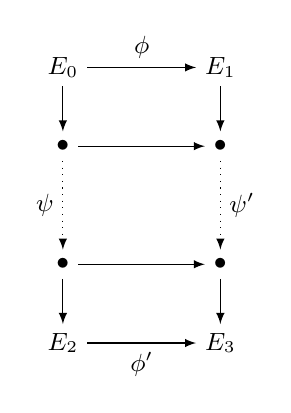
\begin{tikzpicture}
    \small
    \node (E0) at (0,0) {$E_0$};
    \node (E1) at (2,0) {$E_1$};
    \node (Ee0) at (0,-1) {$\bullet$};
    \node (Eo0) at (2,-1) {$\bullet$};
    \node (Ee1) at (0,-2.5) {$\bullet$};
    \node (Eo1) at (2,-2.5) {$\bullet$};
    \node (E2) at (0,-3.5) {$E_2$};
    \node (E3) at (2,-3.5) {$E_3$};

    \draw[-latex]
    (E0) edge node[above] {$\phi$} (E1)
    (Ee0) edge (Eo0)
    (Ee1) edge (Eo1)
    (E2) edge node[below] {$\phi'$} (E3)
    (E0) edge (Ee0)
    (E1) edge (Eo0)
    (Ee1) edge (E2)
    (Eo1) edge (E3);
    \draw[dotted,-latex]
    (Ee0) edge node[left] {$\psi$} (Ee1)
    (Eo0) edge node[right] {$\psi'$} (Eo1);
  \end{tikzpicture}
\end{equation*}
\caption{An SIDH ladder.} \label{fig:ladder}
\end{figure}

Additionally, one may glue SIDH squares both vertically and
horizontally, thus freeing the protocol from the constraint of having
the isogeny degrees divide $p+1$.


\subsection{SIDH signatures}

The Fiat-Shamir heuristic can be used to make sigma protocols non-interactive.
%From the point of view of signatures it is most efficient to stick with the simplest protocols.
The basic DFJP protocol from Section~\ref{sec:DFJP} has been used to construct a signature scheme in Yoo et al~\cite{YAJJS17} and~\cite{GPS20}, based on the hardness of the relation \R[isog]. \LDF{\R[SIDH]?}
These schemes are no longer secure, due to the attacks on SIDH, but it is fairly straightforward to construct secure signatures based on any of the protocols with ternary challenges above.



%\subsection{Other approaches}
%
%k-SIDH?
%
%\LDF{Hmmm, not really a PoK, is it?}
%\SG{Agree. Delete this}


\subsection{Questions and perspectives}

We now discuss some of the limitations of the protocols above.

\paragraph{Efficiency.}
Using ternary challenges comes at a cost: to achieve soundness error of $2^{-\lambda}$, one needs $\lambda/(\log_2(3)-1)$ iterations, each iteration computing one or more SIDH squares.
A major open problem is whether there exist protocols for any of these relations with small soundness error, possibly exponentially small.
SQISign, presented in Section~\ref{sec:SQIsign}, will provide a beginning of an answer for the relation $\R[isog]$.

\paragraph{Statistical ZK for \R[deg].}
Currently, there appears to be a tension between soundness and
zero-knowledge for \R[deg]: the ``flipping the SIDH square'' technique
of Section~\ref{sec:R-deg} is incompatible with the ``SIDH ladders''
of Section~\ref{sec:from-comp-stat}.  Indeed, in an SIDH ladder the
$D$-torsion is not anymore defined over the base field, and it is thus
not possible to define the torsion bases $(P_2,Q_2),(P_3,Q_3)$ used to
prove special soundness for \R[deg].

It is an interesting question to find alternative representations for
$D$-torsion bases that are compatible with SIDH ladders.
%\LDF{Actually, I think I know how to do this, but I'm not sure I want to do it!}

\paragraph{ZK for \R[isog]}
All the protocols we presented so far appear to leak $\deg(\phi)$ to
the verifier when responding with the isogeny $\phi'$ parallel to
$\phi$. It seems thus difficult to make them zero-knowledge for
\R[isog], rather than \R[deg].

Is is equally interesting to find a zero-knowledge protocol,
computationally or statistically, for the \R[isog] relation in the case where the endomorphism ring is not known.
